\documentclass{article}
\usepackage[utf8]{inputenc}
\usepackage{multicol}
\usepackage{listings}
\usepackage{geometry}
\usepackage{color}
\usepackage{float}
\setlength{\belowcaptionskip}{-10pt}
\setlength{\abovecaptionskip}{-30pt}
\floatstyle{boxed} 
\restylefloat{figure}
\usepackage{graphicx}
\definecolor{codegreen}{rgb}{0,0.6,0}
\definecolor{codegray}{rgb}{0.5,0.5,0.5}
\definecolor{codepurple}{rgb}{0.58,0,0.82}
\definecolor{backcolour}{rgb}{0.95,0.95,0.92}

\lstdefinestyle{mystyle}{
	backgroundcolor=\color{backcolour},   
	commentstyle=\color{codegreen},
	keywordstyle=\color{blue},
	numberstyle=\tiny\color{codegray},
	stringstyle=\color{codepurple},
	basicstyle=\footnotesize,
	breakatwhitespace=false,         
	breaklines=true,                 
	captionpos=b,                    
	keepspaces=true,                 
	numbers=left,                    
	numbersep=5pt,                  
	showspaces=false,                
	showstringspaces=false,
	showtabs=false,                  
	tabsize=2
}

\lstset{style=mystyle}
\title{Machine Learning\\ Home Work 01}
\author{aqeel labash}
\date{13 February 2016}
\geometry{
	a4paper,
	total={170mm,257mm},
	left=10mm,
	top=5mm,
}
\begin{document}
	
	\maketitle
	\section*{\centering{First Question}}
	\subsection*{\centering{First(a)}}
	To replace numerical codes to labels I used factor. Factor method replace the value that match with corresponding label (original values , values to be matched, Corresponding labels).(\textbf{Note: }I initiated all the vectors on the fly )
	\begin{lstlisting}[language=R]
	#Convert Landmass
	data$landmass <- factor(data$landmass,c(1:6),c("N.America", "S.America", "Europe", "Africa", "Asia", "Oceania"))
	#Convert zone
	data$zone <- factor(data$zone,c(1:4),c('NE','SE','SW','NW'))
	unique(data$language)
	#Concert Language
	data$language<- factor(data$language,c(1:10),c('English', 'Spanish', 'French','German','Slavic','Other Indo-European', 'Chinese', 'Arabic','Japanese/Turkish/Finnish/Magyar', 'Others'))
	#Convert Religion
	unique(data$religion)
	data$religion = factor(data$religion,c(0:7),c('Catholic', 'Other Christian','Muslim','Buddhist',
	'Hindu','Ethnic','Marxist','Others'))
	\end{lstlisting}
	\textbf{Figure 1} shows a comparison between religion in number of countries.
	\begin{figure}[H]
		\begin{center}
			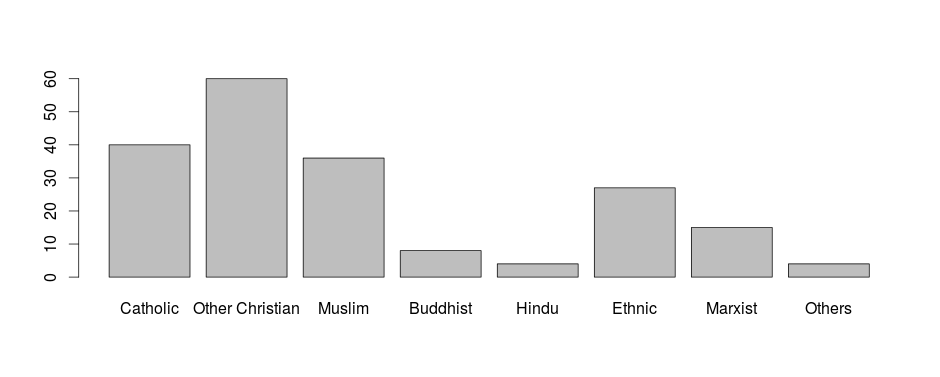
\includegraphics[scale=0.5]{barplotreligion.png} %Image name here.
		\end{center}
		\caption{Countries Religion} %Figure name here.
	\end{figure}
	
	\textbf{Figure 2} shows a comparison between landmasses in number of countries.(how many countries in each landmass)
	\begin{figure}[H]
		\begin{center}
			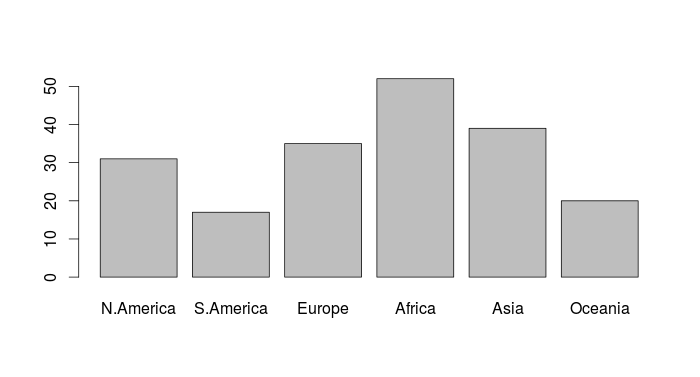
\includegraphics[scale=0.7]{barplotlandmass.png} %Image name here.
		\end{center}
		\caption{Countries landmass} %Figure name here.
	\end{figure}
	\textbf{Figure 3} shows a comparison between languages in number of countries.(how many countries has that language as official)
	\begin{figure}[H]
		\begin{center}
			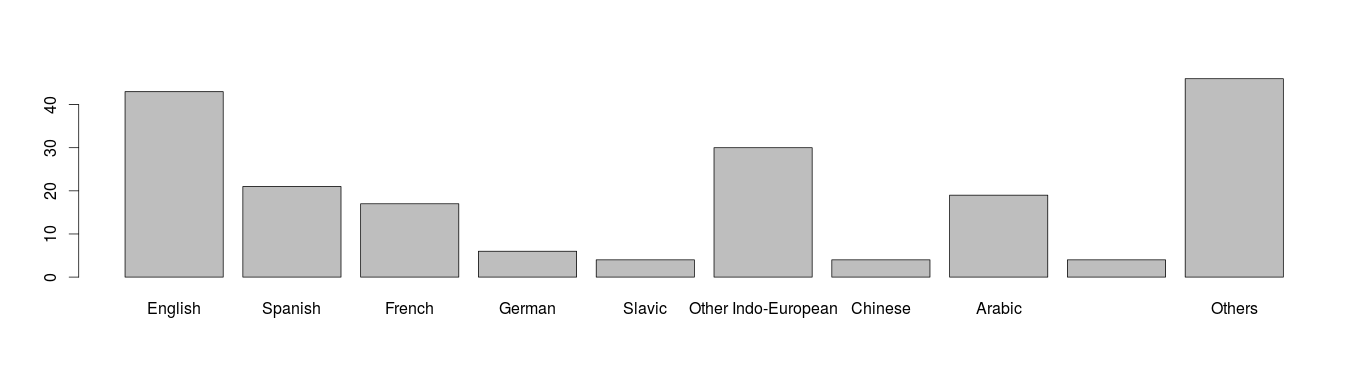
\includegraphics[scale=0.3]{barplotlanguages.png} %Image name here.
		\end{center}
		\caption{Countries landmass} %Figure name here.
	\end{figure}
	The previous plots where done by the following code where the data converted to a table and then the plot has been done.
	\begin{lstlisting}[language=R]
	#religion barplot 
	barplot(table(data$religion))
	#landmass barplot
	barplot(table(data$landmass))
	#language barplot
	barplot(table(data$language))
	\end{lstlisting}
	
	\subsection*{\centering{First(b)}}
	(I interpreted this task to show how religion \& landmass effect the area and population)
	For this task first I filtered the data to Africa and Europe only.Then I dropped the levels so only Africa and Europe will show up in the plot
	\begin{lstlisting} [language=R]
	#First Isolate the data I want to work on for this question.
	importadata = subset (data,landmass=="Europe" | landmass =="Africa")
	
	#drop levels of landmass (landmass other than(Europe , Africa) won't show up in the plot)
	importadata$landmass <- droplevels(importadata$landmass)
	#plot area vs landmass
	\end{lstlisting}
	as shown in figure 4 we can notice that Africa countries has more area than Europe countries. As well we can notice in Africa we have two exceptions (Sudan and Algeria) (\textbf{Soviet Union in dataset still exist and it's in Asia})
	\begin{figure}[H]
		\begin{center} 
			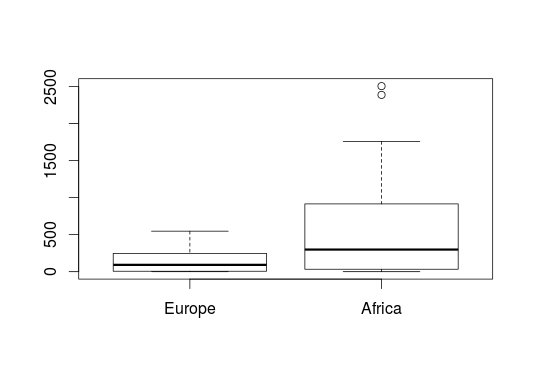
\includegraphics[scale=0.9]{boxplotareavslandmass.png} %Image name here.
		\end{center}
		\caption{Countries area corresponding to landmass(Europe and Africa)} %Figure name here.
	\end{figure}
	Figure 5 shows that countries in Europe has more population than African countries.
	\begin{figure}[H]
		\begin{center}
			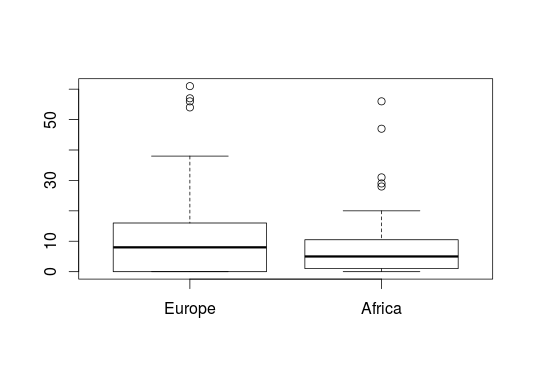
\includegraphics[scale=0.95]{boxplotpopulationvslandmass.png} %Image name here.
		\end{center}
		\caption{Countries population corresponding to landmass(Europe and Africa)} %Figure name here.
	\end{figure}
	Now to see the area and population dependency on religion\\
	In Figure 6 we clearly notice that Hindu countries has wide area. But in the same time it's median is very low which mean that countries above the median is very distributed. Marxist has high median which mean that countries above the median is not very distributed. 
	\begin{figure}[H]
		\begin{center}
			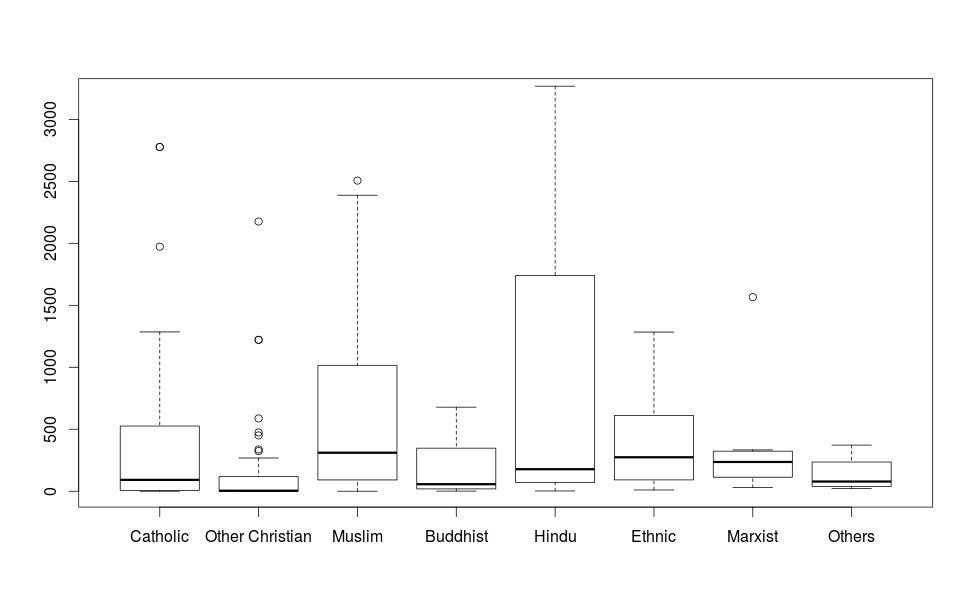
\includegraphics[scale=0.5]{boxplotareavsreligion.png}
		\end{center}
		\caption{Countries area corresponding to religion} %Figure name here.
	\end{figure}
	Just to clarify the previous figure I calculated number of Hindu \& Marxist \& Muslim countries and I found that there is 4 Hindu countries which explain why it's was very distributed.There is 36 Muslim countries and we can tell that Muslim countries has high probability to have more area than (Other Christian) countries.
	\begin{lstlisting}[language=R]
	#Number of Hindu Countries
	length(subset(data,religion=='Hindu')$landmass)
	#Number of Marxist Countries
	length(subset(data,religion=='Marxist')$landmass)
	#Number of Muslim Countries
	length(subset(data,religion=='Muslim')$landmass)
	\end{lstlisting}
	In figure 7 we can see boxplot for Countries popluation corresponding to religion but to make it more clear I'll minimize the range in figure 8.
	\begin{figure}[H]
		\begin{center}
			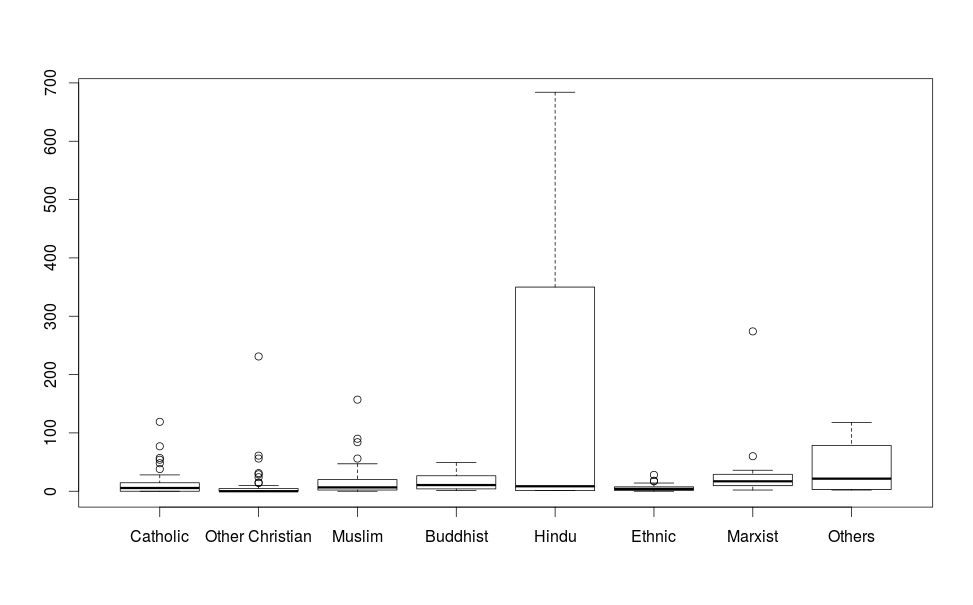
\includegraphics[scale=0.5]{boxplotpopulationvsreligion.png}
		\end{center}
		\caption{Countries population corresponding to religion}
	\end{figure}
	In figure 8 we can see that (Hindu,Others) countries have high population and Hindu countries has high probability to have high population over other religion.
	\begin{figure}[H]
		\begin{center}
			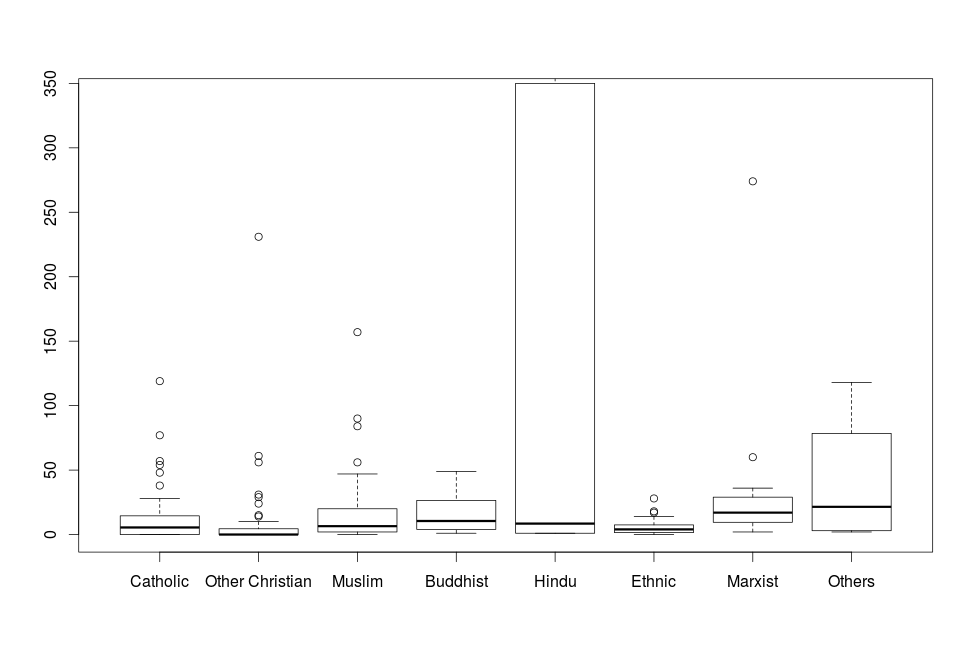
\includegraphics[scale=0.5]{boxplotpopulationvsreligionminimized.png}
		\end{center}
		\caption{Countries population corresponding to Religion (mimized)}
	\end{figure}
	The Previous plots were generated by this code.
	\begin{lstlisting}[language=R]
	#plot area vs landmass
	boxplot(area ~ landmass,data=importadata)
	
	#plot popluation vs landmass
	boxplot(population ~landmass,data=importadata)
	
	#plot area vs religion
	boxplot(area ~religion,data,ylim=c(0,3200))
	
	#plot population vs religion
	boxplot(population ~religion,data,ylim=c(0,680))
	
	#plot population vs religion (minimze scale)
	boxplot(population ~religion,data,ylim=c(0,340))
	\end{lstlisting}
	\textbf{Note:}the domain (0,3200) and (0,680) were selected as less as possible to have a better view over the plots
	\subsection*{\centering{First(c)}}
	To compute quantiles I created vector contain values from 0.1 to 0.9 (because the question requested from 10\% to 90\%).After that computation were done for area,population and density (density =\(\frac{population*1000000}{area*1000}\)) by the following code:
	\begin{lstlisting}[language=R]
	#Basic Variables
	qlvls = c(1:9)/10
	dataEurope<-subset(data,landmass=="Europe")
	dataAfrica<-subset(data,landmass=="Africa")
	#quantile area 
	quant.Europe.area<-quantile(dataEurope$area,qlvls)
	quant.Africa.area<-quantile(dataAfrica$area,qlvls)
	
	#quantile population
	quant.Europe.population<-quantile(dataEurope$population,qlvls)
	quant.Africa.population<-quantile(dataAfrica$population,qlvls)
	
	#quantile density
	EuropeDensity <- (dataEurope$population*1000000)/(dataEurope$area*1000)
	AfricaDensity <- (dataAfrica$population*1000000)/(dataAfrica$area*1000)
	\end{lstlisting}
	Figure 9 shows that countries in Africa larger and distributed over all quantiles in the other hand Europe not distributed over all quantiles.
	\begin{figure}[H]
		\begin{center}
			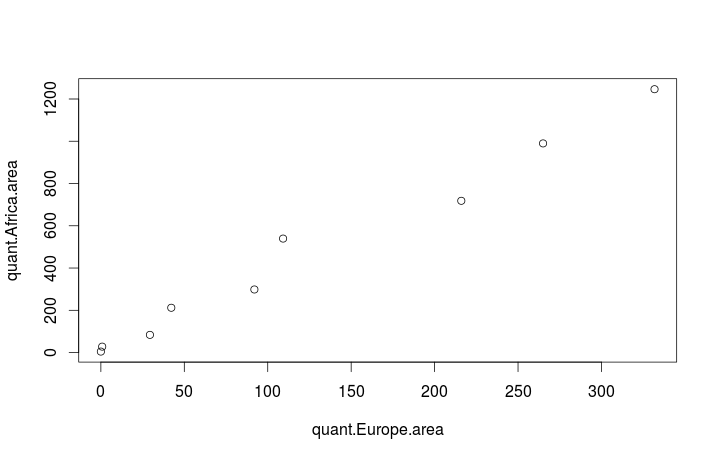
\includegraphics[scale=0.7]{qqplotarea.png}
		\end{center}
		\caption{Countries area in Europe vs Africa}
	\end{figure}
	In figure 9 we can see that Africa countries has more areas than Europe ones.
	\begin{figure}[H]
		\begin{center}
			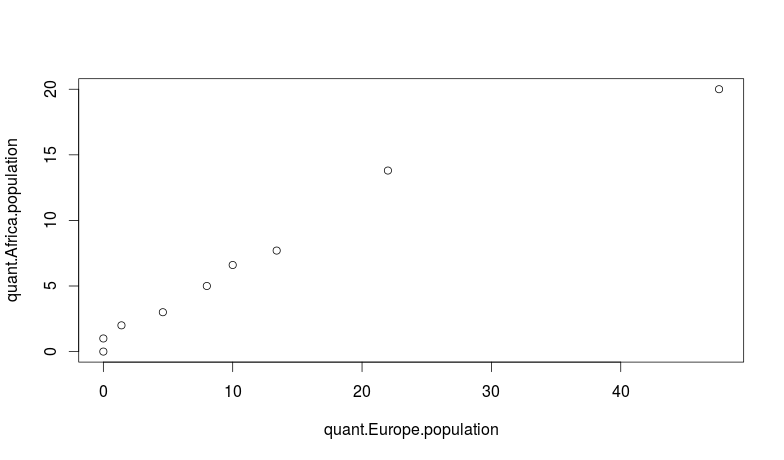
\includegraphics[scale=0.6]{qqplotpopulation.png}
		\end{center}
		\caption{Countries population in Europe vs Africa}
	\end{figure}
	In figure 10 we can observe how Europe countries has more population than African countries.
	\begin{figure}[H]
		\begin{center}
			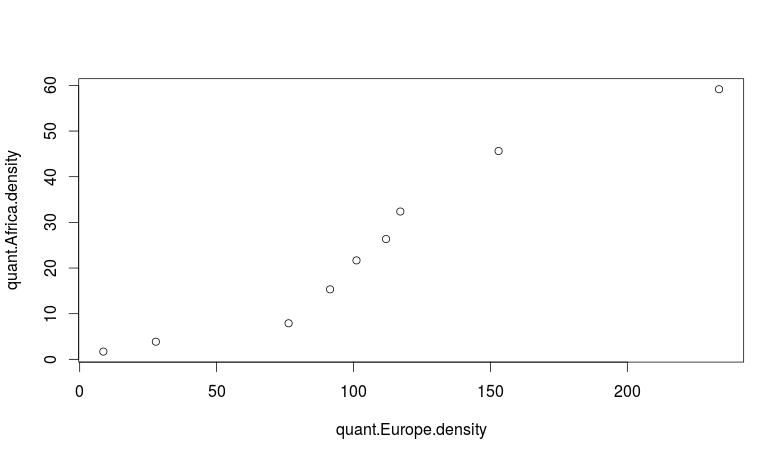
\includegraphics[scale=0.6]{qqplotdensity.png}
		\end{center}
		\caption{Countries density in Europe vs Africa}
	\end{figure}
	In figure 11 it's clearly that Europe has higher density and that's due Africa has larger area but less population as we saw in figure 9\&10
	\subsection*{\centering{First(d)}}
	To get the cover we get number of rows for (Marxist, Muslim , English).\\
	Support we get the number of rows for the condition and the result (Marxist\&red , Muslim\&green , English\& saltires\(>\)0).\\
	Relative Support : Support to total data.\\
	Confidence: Support / Cover. and here is the code used for it:
	\begin{lstlisting}[language=R]
	#Cover
	Marxist.Cover = nrow(subset(data,religion=="Marxist"))
	Muslims.Cover = nrow(subset(data,religion=="Muslim"))
	English.Cover = nrow(subset(data,language=="English"))
	
	#Support
	Marxist.Support = nrow(subset(data,religion=="Marxist" & red=="1"))
	Muslim.Support = nrow(subset(data,religion=="Muslim" & green=="1"))
	English.Support = nrow(subset(data,language=="English"& saltires>0))
	
	#Relative Support
	Marxist.RelativeSupport = Marxist.Support/nrow(data)*100
	Muslim.RelativeSupport = Muslim.Support/nrow(data)*100
	English.RelativeSupport = English.Support/nrow(data)*100
	
	#Confidence 
	Marxist.Confidence = Marxist.Support/Marxist.Cover
	Muslims.Confidence = Muslim.Support/Muslims.Cover
	English.Confidence = English.Support/English.Cover
	\end{lstlisting}
	The result was : \\
	Marxist Cover : 15 , Support : 15 , Relative Support : 7.731959, Confidence : 1.\\
	Muslims Cover : 35 , Support : 26 , Relative Support : 13.40206, Confidence : 0.72\\
	English Cover : 43, Support : 15 , Relative Support : 7.731959, Confidence: 0.3488372\\
	\subsection*{\centering{First(e)}}
	As I understood the question here I need to find the best rules for 3 cases :saltries , crosses , (Sun or star)\\
	\textbf{Saltires}:Firstly I analyzed the data and I noticed that English \& Other Christian were the most common between all saltires.And here is the code:
	\begin{lstlisting}[language=R]
	#analyzing saltires data
	testdata <- subset(data,saltires>0)
	#trying rules
	saltires.English.Support <- nrow(subset(data,language=="English" &saltires>0))
	saltires.English.Confidence <-saltires.English.Support /nrow(subset(data,language=="English" ))
	saltires.OtherChristian.Support<-nrow(subset(data,religion =="Other Christian"&saltires>0))
	saltires.OtherChristian.Confidence<-saltires.OtherChristian.Support/nrow(subset(data,religion=="Other Christian"))
	saltires.Zone.Support <-nrow(subset(data,zone=="NW"& saltires>0))
	saltires.Zone.Confidence<-saltires.Zone.Support/ nrow(subset(data,zone=="NW"))
	\end{lstlisting}
	Using English language as the rule I got :Support : 15, Confidence:0.348837.\\
	Using religion "Other Christian" as the rule I got: Support :16 , Confidence : 0.26.\\
	Using zone "NW" as the rule I got : Support : 7 , Confidence: 0.12.\\
	Obviously English rule got the highest confidence after that the religion and that's as I looked into it it's related to Scotland and saint Andrews.\\
	
	\textbf{Crosses}:I did as before first analyzed the data were it was the same English \& Other Christian \& blue as bottom right color of the flag were most common shared characteristics between the data and here is the code :
	\begin{lstlisting}[language=R]
	#analyzing crosses
	testdata<-subset(data,crosses>0)
	
	#trying rules
	crosses.OtherChristian.Support<-nrow(subset(data,religion=="Other Christian"& crosses>0))
	crosses.OtherChristian.Confidence<-crosses.OtherChristian.Support/nrow(subset(data,religion=="Other Christian"))
	
	crosses.English.Support<-nrow(subset(data,language=="English"& crosses>0))
	crosses.English.Confidence<-crosses.OtherChristian.Support/nrow(subset(data,language=="English"))
	
	crosses.blue.Support<-nrow(subset(data,botright=="blue"&crosses>0))
	crosses.blue.Confidence<-crosses.blue.Support/nrow(subset(data,botright=="blue"))
	
	crosses.zone.Support <-nrow(subset(data,zone=="NE"&crosses>0))
	crosses.zone.Confidence<-crosses.zone.Support/nrow(subset(data,zone=="NE"))
	\end{lstlisting}
	The results were as following : \\
	Using English language as rule : Support : 14 , Confidence: 0.55813.\\
	Using "Other Christian" religion as rule : Support: 24 , Confidence:0.4.\\
	Using blue color for bottom right as rule : Support 17, Confidence : 0.36\\
	Using NE for zone as rule : Support 8, Confidence : 0.87.\\
	Actually here I believe the cross is related to the history of NE zone.So if I have to pick a rule I would pick it event if this rule have small support but with high confidence it's better to go with I believe.\\
	
	\textbf{SunsorStars}:This was hard to analyze and I used a new way to tackle it.First the code then the result.
	\begin{lstlisting}[language=R]
	#analyzing Sunsorstars
	testdata<-subset(data,sunstars>0)
	#Check By Language
	table(testdata$language)
	table(testdata$language)/table(data$language)
	#Check By landmass
	table(testdata$landmass)
	table(testdata$landmass)/table(data$landmass)
	#Check By religion
	table(testdata$religion)
	table(testdata$religion)/table(data$religion)
	#Check By Zone
	table(testdata$zone)
	table(testdata$zone)/table(data$zone)
	\end{lstlisting}
	After executing the above code here is the result :\\
	
	\textbf{Support \& Confidence Language} 
	\begin{flushleft}
		\begin{tabular}{|c|c|c|c|c|c|c|c|c|c|c|}
			\hline
			&English&Spanish&French&German&Slavic&Over Indo-E & Chinese&Arabic&J/T/F/M&Other\\
			\hline
			Support&16&9&8&0&2&10&3&9&2&21\\
			\hline
			Confidence&0.37&0.42&0.47&0.0&0.5&0.33&0.75&0.47&0.5&0.45\\
			\hline
		\end{tabular}
	\end{flushleft}
	\textbf{Support \& Confidence landmass} 
	\begin{flushleft}
		\begin{tabular}{|c|c|c|c|c|c|c|}
			\hline
			&N.America&S.America&Europe&Africa&Asia&Oceania \\
			\hline
			Support&10&8&4&24&20&14 \\
			\hline
			Confidence&0.3225806&0.4705882&0.1142857&0.4615385&0.5128205&0.7000000\\
			\hline
		\end{tabular}
	\end{flushleft}
	\textbf{Support \& Confidence Religion}
	\begin{flushleft}
		\begin{tabular}{|c|c|c|c|c|c|c|c|c|}
			\hline
			&Catholic&Other Christian&Muslim&Buddhist&Hindu&Ethnic&Marxist&Others\\
			\hline
			Support&13&20&17&3&1&13&10&3\\
			\hline
			Confidence&0.3250000&0.3333333&0.4722222&0.3750000&0.2500000&0.4814815&0.6666667&0.7500000\\
			\hline
		\end{tabular}
	\end{flushleft}
	\textbf{Support \& Confidence Zone}
	\begin{flushleft}
		\begin{tabular}{|c|c|c|c|c|}
			\hline
			&NE&SE&SW&NW\\
			\hline
			Support&37&13&9&21\\
			\hline
			Confidence&0.4065934&0.4482759&0.5625000&0.3620690\\
			\hline
		\end{tabular}
	\end{flushleft}
	From the previous results we can see that Using Chinese rule give the highest Confidence but not the highest support. We can't depend on that because it's not supported rule (Same goes for best Confidence in religion rules(Others))\\
	From landmass Oceania has 14 for Support \& 0.7 for Confidence.\\
	In zone SW zone has the best Confidence but yet not the best support compared to landmass rule.\\
	So here I would go with landmass rule for Oceania.It can be explained as common history in Oceania.
	\subsection*{\centering{First(f)}}
	\textbf{For saltires} I merged two rules from previous request to get better result here so the rule is English for language \& Other Christian for religion. and I got Support :15 , Confidence : 0.41.\\
	\textbf{Crosses:} I picked the rule as (zone:SW,language:English,Crosses>0) and I got Support:4,Confidence:0.66.\\
	\textbf{Sunstars:} I used the previous request tables to help me judge so the rule was (language:English,landmass:Oceania,sunstars>0) the result : Support:9,Confidence : 0.75.
	I would pick sunstar as a rule (although it's the same result of previous request),But still it's the one with best Support and accuracy I got up to know.\\
	Here is the code used for this task :
	\begin{lstlisting}[language=R]
	#First (f)
	testdata <- subset(data,saltires>0)
	saltires.EnglishAndOtherChristian.Support <-nrow(subset(data,language=="English"&religion=="Other Christian" & saltires>0))
	saltires.EnglishAndOtherChristian.Confidence <-saltires.EnglishAndOtherChristian.Support /nrow(subset(data,language=="English"&religion=="Other Christian"))
	
	testdata<-subset(data,crosses>0)
	crosses.EnglishAndSW.Support<-nrow(subset(data,zone=="SW"&language=="English"&crosses>0))
	crosses.EnglishAndSW.Confidence <- crosses.EnglishAndSW.Support/nrow(subset(data,zone=="SW" & language =="English"))
	testdata<-subset(data,sunstars>0)
	sunsorstars.EnglishAndOceania.Support <-nrow(subset(data,language=="English"&landmass=="Oceania"&sunstars>0))
	sunsorstars.EnglishAndOceania.Confidence<-sunsorstars.EnglishAndOceania.Support/nrow(subset(data,language=="English"&landmass=="Oceania"))
	\end{lstlisting}
	\subsection*{First(g)}
	For this question I'll the feature if there is green color in a flag then it's a Muslim country.\\
	\begin{tabular}{|c|c|c|}
		\hline
		&Predicted positives&Predicted negatives\\
		\hline
		Labelled positives&26&65\\
		\hline
		Labelled negatives&10&93\\
		\hline
	\end{tabular}\\
	To Change the positive class (as I understood we have to take the opposite feature) The feature become if there is no green color then it's not a Muslim country.\\
	\begin{tabular}{|c|c|c|}
		\hline
		&Predicted positives&Predicted negatives\\
		\hline
		Labelled positives&93&10\\
		\hline
		Labelled negatives&65&26\\
		\hline
	\end{tabular}\\
	We can notice that the result is the same just the places changed depending on what we consider positive ,negative.
	\begin{lstlisting}[language=R]
	#First(G)
	#I USED THE CODE FROM PREVIOUS YEAR PRACTICE SESSION JUST CHANGED THE PARAMETERS
	# Elements of a confusion matrix
	true.positives = nrow(subset(data, green==1 & religion == "Muslim"))
	true.negatives = nrow(subset(data, green ==0 & religion != "Muslim"))
	false.positives = nrow(subset(data, green ==0 &  religion == "Muslim"))
	false.negatives = nrow(subset(data,  green==1& religion != "Muslim"))
	
	confusion.matrix <- rbind(c(true.positives, false.negatives), c(false.positives, true.negatives))
	colnames(confusion.matrix) <- c("Predicted positives", "Predicted negatives")
	rownames(confusion.matrix) <- c("Labelled positives", "Labelled negatives")
	confusion.matrix
	#Opposite
	true.positives = nrow(subset(data, green==0 & religion != "Muslim"))
	true.negatives = nrow(subset(data, green ==1 & religion == "Muslim"))
	false.positives = nrow(subset(data, green ==1 &  religion != "Muslim"))
	false.negatives = nrow(subset(data,  green==0& religion == "Muslim"))
	
	confusion.matrix <- rbind(c(true.positives, false.negatives), c(false.positives, true.negatives))
	colnames(confusion.matrix) <- c("Predicted positives", "Predicted negatives")
	rownames(confusion.matrix) <- c("Labelled positives", "Labelled negatives")
	confusion.matrix
	\end{lstlisting}
	\section*{\centering{Second Question}}
	\subsection*{\centering{Second(a)}}
	I depended on function sample for this request and here is the code:
	\begin{lstlisting}[language=R]
	#Second (a)
	GetSamples<-function(X,n){
	S <- sample(x =  X,size =  n,replace = TRUE)
	print(min(S))
	print (mean(S))
	return (S)
	}
	values<-c(1:10000)
	GetSamples(values,10)
	\end{lstlisting}
	\subsection*{Second(b)}
	For this task I updated the previous function not to SPAM the screen with output.Used sd() function to calculate the deviation.Here is the code after it the result.
	\begin{lstlisting}[language=R]
	#Second(b)
	#write the function without printig not to spam
	GetSamples2<-function(X,n){
	S <- sample(x =  X,size =  n,replace = TRUE)
	return (S)
	}
	#define value containers 
	meanVector<-c(1:1000)
	minVector<-c(1:1000)
	
	
	for (i in 1:1000)
	{
	#Get sample 
	#n = 1,10,100,1000,10000 
	currentSample = GetSamples2(values,10000)
	#calculate current min,mean
	meanVector[i] = mean(currentSample)
	minVector[i]=min(currentSample)
	}
	average.mean=mean(meanVector)
	average.min=mean(minVector)
	sd(meanVector)
	sd(minVector)
	\end{lstlisting}
	The result of previous code was as following :\\
	
	\begin{tabular}{|c|c|c|c|c|}
		\hline
		&\multicolumn{2}{c|}{Standard Deviation }&\multicolumn{2}{c|}{Average}\\
		\hline
		Size&mean&min&mean&min\\
		\hline
		1&2933.957&2933.957&4973.313&4973.313\\
		\hline
		10&908.7539&878.4209&5065.1008&952.722\\
		\hline
		100&289.9641&99.06789&4989.76864&99.765\\
		\hline
		1000&88.99537&9.717406&5001.901446&10.729\\
		\hline
		10000&28.593&1.023292&5000.2225452&1.589\\
		\hline 
	\end{tabular}\\
	
	Previous table tell us, the larger element we take the more accurate our answer will be.In figure 12 and 13(better view) we can see that the more n size increase the less deviation we get.
	\begin{figure}[H]
		\begin{center}
			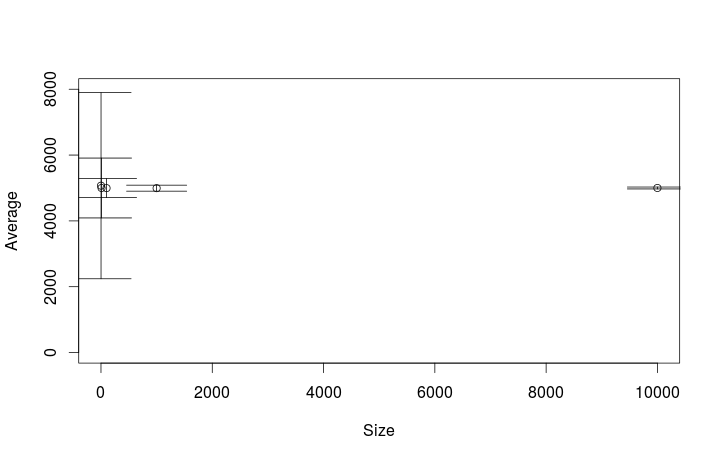
\includegraphics[scale=0.7]{plotmeanall.png}
		\end{center}
		\caption{Shows the deviation of mean average vs n size}
	\end{figure}
	\begin{figure}[H]
		\begin{center}
			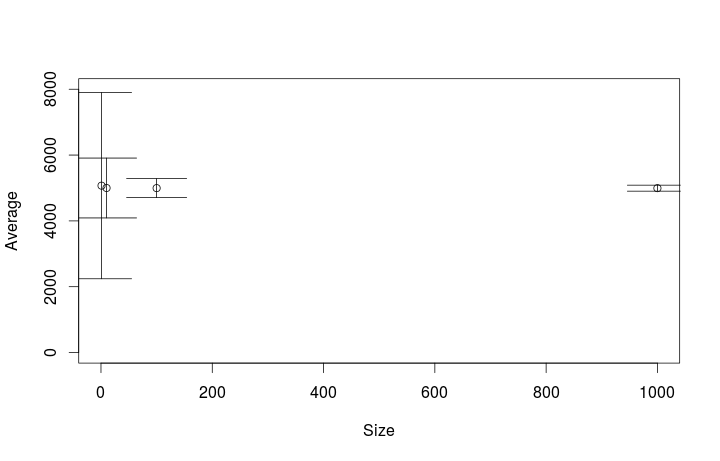
\includegraphics[scale=0.6]{plotmean4.png}
		\end{center}
		\caption{More clear view of deviation over mean average vs n size}
	\end{figure}
	The same for min value as shown in figure 14,15(better view), the more samples we take the less deviation we have.
	\begin{figure}[H]
		\begin{center}
			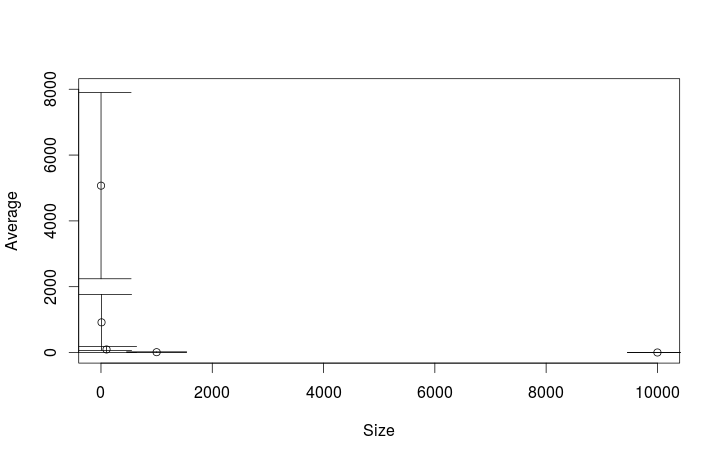
\includegraphics[scale=0.7]{plotminall.png}
		\end{center}
		\caption{Shows deviation over min average vs n size}
	\end{figure}
	\begin{figure}[H]
		\begin{center}
			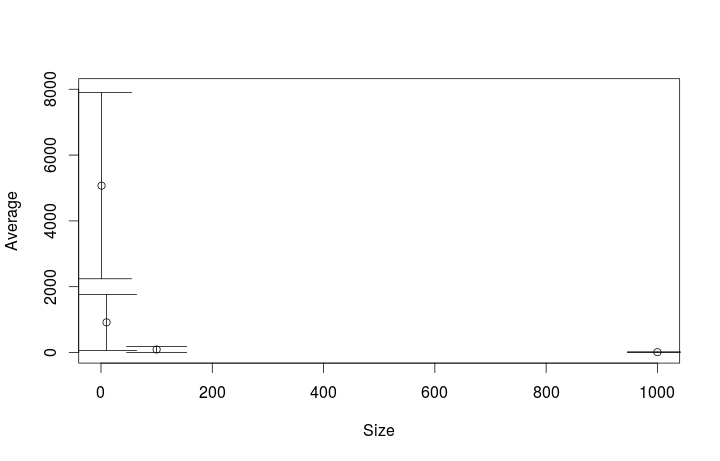
\includegraphics[scale=0.7]{plotmin4.png}
		\end{center}
		\caption{Same as figure 14 but focusing on first 4 n sizes}
	\end{figure}
	Here is the Code is used for this task:\\
	\begin{lstlisting}[language=R]
	#Second(b)
	values<-c(1:10000)
	#write the function without printig not to spam
	GetSamples2<-function(X,n){
	S <- sample(x =  X,size =  n,replace = TRUE)
	return (S)
	}
	#define value containers 
	meanVector<-c(1:1000)
	minVector<-c(1:1000)
	meav <- vector(mode="numeric", length=0)
	miav <- vector(mode="numeric", length=0)
	mesd <- vector(mode="numeric", length=0)
	misd <- vector(mode="numeric", length=0)
	for (n in c(1,10,100,1000,10000))
	{
	
	for (i in 1:1000)
	{
	#Get sample 
	#n = 1,10,100,1000,10000 
	currentSample = GetSamples2(values,n)
	#calculate current min,mean
	meanVector[i] = mean(currentSample)
	minVector[i]=min(currentSample)
	}
	meav <- c(meav,mean(meanVector))
	miav <- c(miav,mean(minVector))
	mesd <- c(mesd,sd(meanVector))
	misd <- c(misd,sd(minVector))
	
	}
	#THIS CODE WHERE COPIED FROM THIS SOURCE :http://stackoverflow.com/questions/15063287/add-error-bars-to-show-standard-deviation-on-a-plot-in-r
	#I CHANGED THE VALUES TO FIT WHATS REQUESTED IN THE QUESTION
	#prepare data for (mean , min one of them each time )
	d = data.frame(
	x  = c(1,10,100,1000,10000)
	, y  = miav
	, sd = misd
	)
	
	##install.packages("Hmisc", dependencies=T)
	library("Hmisc")
	
	# add error bars (without adjusting yrange)
	plot(d$x, d$y, type="n",ylim=c(0,8000),xlim = c(0,1000),xlab = "Size",ylab = "Average")
	with (
	data = d
	, expr = errbar(x, y, y+sd, y-sd, add=T, pch=1, cap=.1)
	)
	\end{lstlisting}
	
	\subsection*{Second(c)}
	For this task I used the exact code from previous task after changing the sample function as following : 
	\begin{lstlisting}[language=R]
	GetSamples2<-function(X,n){
	S <- sample(x =  X,size =  n,replace = FALSE)
	return (S)
	}
	\end{lstlisting}
	Firstly here is the table of the results : \\
	\begin{tabular}{|c|c|c|c|c|}
		\hline
		&\multicolumn{2}{c|}{Standard Deviation }&\multicolumn{2}{c|}{Average}\\
		\hline
		Size&mean&min&mean&min\\
		\hline
		1&2909.84151&2909.841512&4959.063&4959.063\\
		\hline
		10&878.72027&793.918030&4983.674&889.157 \\
		\hline
		100&293.56768&91.638599&5006.395&97.378\\
		\hline
		1000&86.95006&9.627084&4997.647&10.044\\
		\hline
		10000&0.00000&0.000000&5000.500&1.000\\
		\hline 
	\end{tabular}\\
	Using sampling with out replacement get better results and less deviation in most cases.The following is the visualization with error bars.Two figures for each (mean,min) one with all n sizes, and the other one after minimizing x scope to get better view.\\
	
	\begin{figure}[H]
		\begin{center} 	
			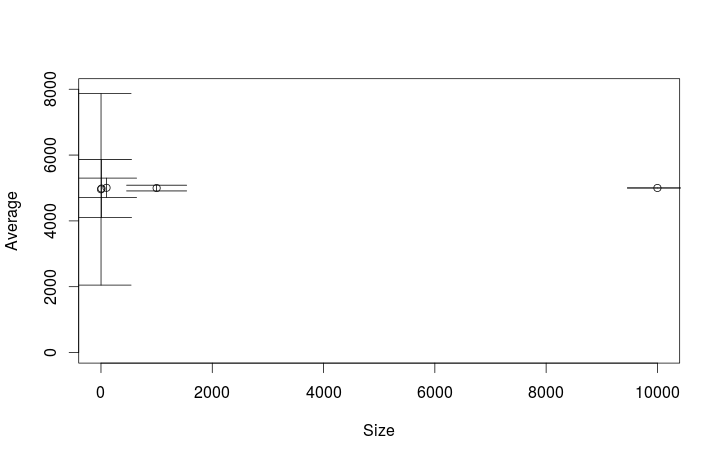
\includegraphics[scale=0.7]{plotmeanallno.png}
		\end{center}
		\caption{Deviation (mean average vs n size )without replacement}
	\end{figure}
	
	\begin{figure}[H]
		\begin{center}
			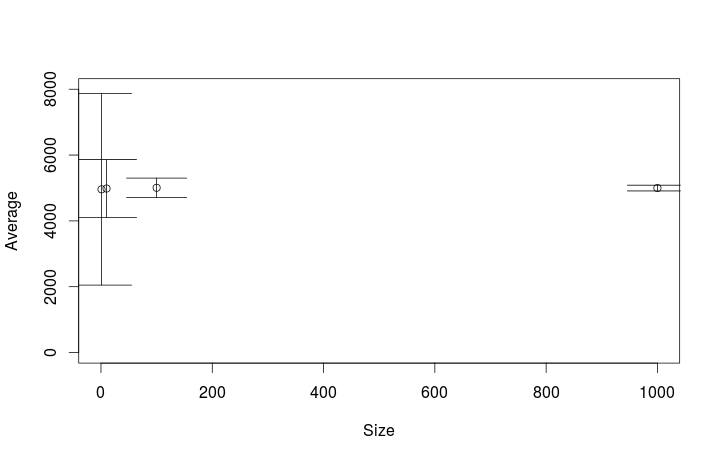
\includegraphics[scale=0.7]{plotmean4no.png}
		\end{center}
		\caption{Deviation (mean average vs n size )without replacement(clearer view)}
	\end{figure}
	
	\begin{figure}[H]
		\begin{center}
			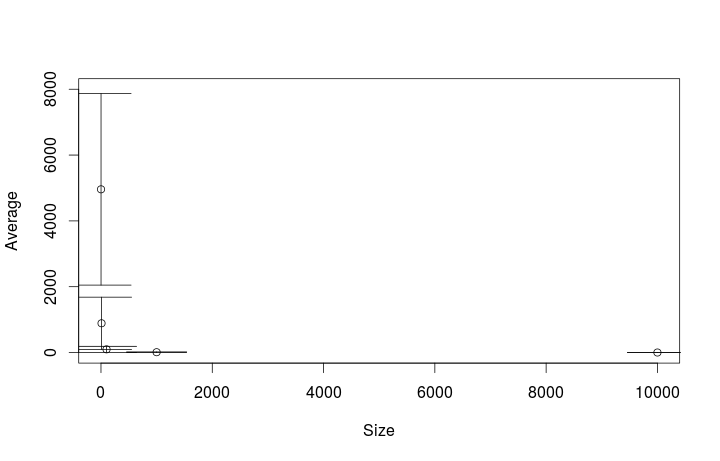
\includegraphics[scale=0.7]{plotminallno.png}
		\end{center}
		\caption{Deviation (min average vs n size )without replacement}
	\end{figure}
	
	\begin{figure}[H]
		\begin{center}
			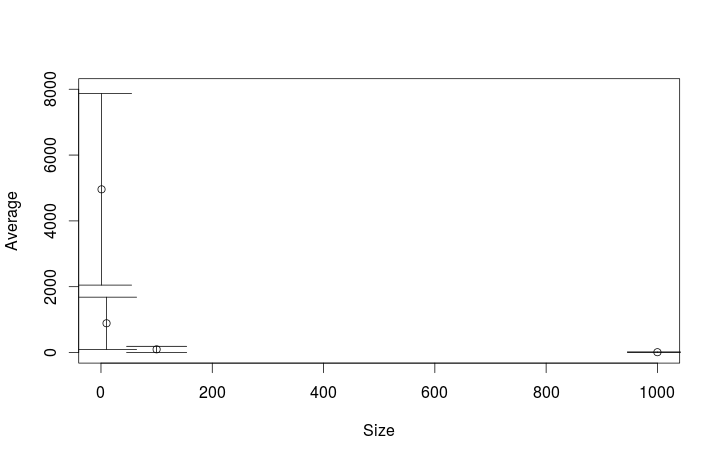
\includegraphics[scale=0.7]{plotmin4no.png}
		\end{center}
		\caption{Deviation (min average vs n size )without replacement(clearer view)}
	\end{figure}
	Comparing the previous figures with ones in (Second question (b)) won't show much difference.That's because the difference is small compared to the scale of the axis. But the comparison by table values is clear.
	\section*{Third Question}
	\subsection*{Third(a)}
	The Code for this question : \\
	\begin{lstlisting}[language=R]
#Third Question (a)
rm (list = ls())
RateFunction<-function (years=20)
{
rates<-vector(mode = "numeric",length = 0)
mean=2
sd =0.5
for (i in c(1:years))
{
#this is not the first round
if (i>1)
{
#If previous rate larger or equal 1 mean =2
if (rates[i-1]>=1)
{
mean=2
}
#If Previous rate less than 1
else if (rates[i-1]<1)
{
mean =0
}
}
#calculate the new rate.
print (mean)
currentrate = rnorm(1,mean = mean,sd = sd)
#Fix the current Rate :
if (currentrate<0)
{
currentrate=0
}
#Fix the rate
rates<-c(rates,currentrate)
}
return (rates)
}
plot(c(1:20),RateFunction(years = 20),type = "l")
	\end{lstlisting}
\begin{figure}[H]
	\begin{center}
	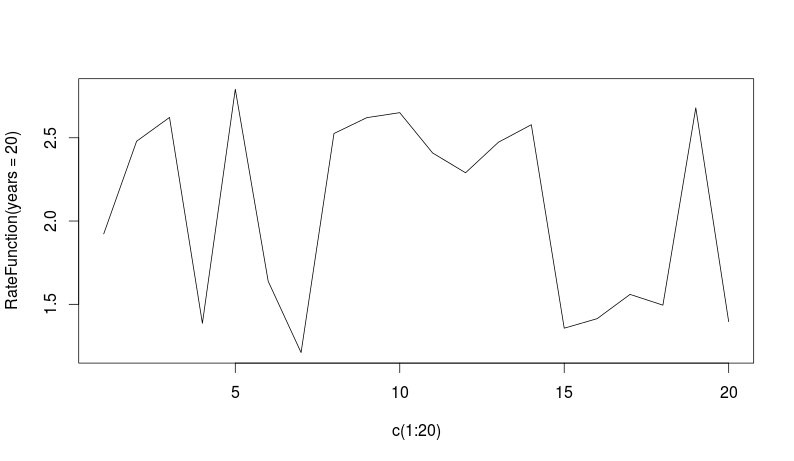
\includegraphics[scale=0.6]{plotrate.png}
	\end{center}
\caption{The Rate value for each year}
\end{figure}
	\subsection*{Third(b)}
Under Construction :D
	\subsection*{Third(c)}
	\subsection*{Third(d)}
	\section*{Fourth Question}
	\subsection*{Fourth(a)}
	\subsection*{Fourth(b)}
	\subsection*{Fourth(c)}
\end{document}
